\documentclass{article}
\usepackage[utf8]{inputenc}
\usepackage{graphicx}
\usepackage[a4paper, total={6in, 9in}]{geometry}
\usepackage{amsmath}
\usepackage{steinmetz}
\usepackage{booktabs}
\usepackage{datatool}
\usepackage[scr]{rsfso}
\newcommand{\Laplace}{\mathscr{L}}

\graphicspath{ {./figures/} }
 
\title{PHYS410 - Homework 2}
\author{Name: Brendan Lai, Student Number: 19241173}
\date{Due: November 4th, 2022}
  
\begin{document}
  
\maketitle
  
\tableofcontents

\section{Homework Objective}
This homework investigates the implementation of a fourth order Runge Kutta solution. It also dives into the associated errors of these solutions.

\section{Theory}

\subsection{Euler's and Fourth Order Runge-Kutta Methods}
This sections analyzes the background of the fourth order Runge-Kutta method.\\
Before we dive into the Runge-Kutta method it is useful to know the background of Euler's method to motivate Runge-Kutta. The approach of Euler's method is based on a Taylor Series expansion (as most things so far). Considering the basic ODE $$y'(x) = f(x,y)$$ 
We see the following Taylor Series expansion:\\
$$y(x) = y(x_0) + (x - x_0) y'(x_0) + \frac{1}{2}(x - x_0)^2 y''(x_0) + ...$$
\\
Further, if we look at higher derivations it gets messy with regards to all the necessary partial derivatives to be calculated. As a result, generally the first two terms of the Taylor Series expansion is what we retain resulting in: $$y(x) = y(x_0) + (x - x_0) y'(x_0)$$
\\
This gives: $$y(x) \approx y(x_0) + (x - x_0)y'(x_0) = y(x_0) + (x-x_0)f(x_0, y_0)$$
\\
Lastly, the "Forward" form of Euler's method is: $$y(x_0 + h) = y(x_0) + h*f(x_0,y_0) = y_0 + h f_0$$
\\
This basic algorithm then takes repeated steps, possibly adjusting step size until the integration limit is reached and in this case the accuracy is $O(h)$ global error and $O(h^2)$ per step error. Obviously, with this accuracy it is imperfect and is generally not used which brings us then to our Runge-Kutta method.\\
\\
Improving Euler's method can be done three different ways: 
\begin{enumerate}
    \item Use a higher order Taylor Series.
    \item Linear multi-step methods, use data from previous time steps to cancel terms in the truncation error.
    \item Runge-Kutta: Use intermediate points within one time step.
\end{enumerate}
\\
With this information the fourth order Runge-Kutta method is one of the most popular solutions in which we define intermediate function evaluations. Note that there are also an infinite number of possible Runge-Kutta methods however we will use the following one which is most used. It is defined as below:\\
\begin{align*}
    f_0 &= f(x_0, y_0)\\
    f_1 &= f(x_0 + \frac{h}{2}, y_0 + \frac{h}{2}f_0)\\
    f_2 &= f(x_0 + \frac{h}{2}, y_0 + \frac{h}{2}f_1)\\
    f_3 &= f(x_0 + h, y_0 + hf_2)\\
\end{align*}
With these intermediate function evaluations and the previous function value use these to evaluate the next value with the following equation:\\
\begin{align*}
    y(x_0 + h) = y_0 + \frac{h}{6}(f_0 + 2f_1 + f_2 + f_3) \qquad\qquad\qquad (1)
\end{align*}

\subsection{Simple Harmonic Oscillator}
One of the system of ODEs that is used extensively through this homework is the simple harmonic oscillator. This is based on the second order differential equation. $$\frac{d^2 x(t)}{dt^2} = -x(t)$$\\
Using some algebra we are able to convert this second order differential equation into a system of first order differential equations. \\
\\
Let $x_1 = x(t)$ and $x_2 = \frac{dx(t)}{dt}$. With this we get the following system of ODEs:
\begin{align*}
    \frac{dx_1(t)}{dt} &= x_2(t)\\
    \frac{dx_2(t)}{dt} &= -x_1(t)
\end{align*}
\\
This system of ODEs is one we use for both quesitons 1 and 2 when analyzing the Runge-Kutta step on it's own as well as when looking at the full implementation of the fourth order Runge-Kutta method.\\
\\
There are many ways to solve this second order differential equation. One of which is provided below to derive the analytical  using Laplace Transforms. $$\Laplace(x'' + x) = s^2 \Laplace x - s x_0 - x'_0 + \Laplace x = 0$$\\
Noting that: $$\Laplace x = \frac{s x_0 + x'_0}{s^2 + 1}$$\\
Thus, the analytical solution is found referring to the tables for Laplace Transforms.$$x(t) = x_0 cos(t) + x'_0 \sin(t)$$

\subsection{Van der Pol Oscillator}
The Van der Pol equation was derived when experimenting with oscillations in a vacuum tube triode circuit. He found that the interesting behaviour in this phenomena could be described with the following second order differential equation. $$\frac{d^2x}{dt^2} + a(x^2 - 1) \frac{dx}{dt} + x = 0$$\\
\\
Once again to handle the second order differential equation we define new variables to convert this into a system of first order differential equations. Letting $x_1 = x(t)$ and $x_2 = x'(t)$ we get the following: 
\begin{align*}
    \frac{dx(t)}{dt} &= x_2\\
    \frac{dx_2(t)}{dt} &= -x_1 - a(x_1^2 - 1) x_2 + b \sin(\omega t)
\end{align*}
\\
This is the system of ODEs we use in problem 2 to analyze both the displacement over time as well as the phase space evolution. Note too that in our implementation later on we set b = 0 and as a result the second term in the second equation in our system of ODEs is zero.

\subsection{Local Step Error}
One way to analyze the local step error is to understand the global step error as they are inherently related. This makes sense because for a complete scheme it would make sense that the degree of each step giving rise to the full scheme affects its results. \\
\\
Defining the order global error as $p$ and the order of the local error as $q$ it can be then determined that the relationship between $p$ and $q$ is $ p = q - 1$ when the numerical method is stable. This is: $$O(\Delta t^p) = O(\Delta t ^{q-1})$$
The other way to analyze local error is to check the step errors for a set of data points and then compare these results against different errors for the same points on different levels. From this we would then also expect our ratio of errors to meet the expectations defined above. \\
\\
So to verify our local step order is fifth order then we could analyze the global error checking if it is fourth order. And then verify our assumption by selectively analyzing errors for different levels and ensuring that these errors are fifth order which maintains the relationship between step and global errors as discussed.

\subsection{Adpative Step Size Runge-Kutta Method}
This background is related to the adaptive step size implementation in problem 3 of this homework. The fourth order Runge-Kutta integrator varies the step size in response to the estimated local solution error. The error estimation is given as the following analysis.\\
\\
The basis of this method is focusing on what we define as a coarse step which is our normal $\Delta t$ step and comparing the results of taking two steps at $\Delta t / 2$ to get to the same next point and then adjusting our $\Delta t$ accordingly after this. Letting $t_0$ be the current time step we are looking at during the integration and $\Delta t$ as the step size we see the following: $$y_{coarse} (t_0 + \Delta t)\approx y_{exact} (t_0 + \Delta t) + k(t_0)(\Delta t^5)$$. 
In this instance $k(t_0)$ is some function of time. Also we define that the local error is: $$e_{local} = y_{coarse} - y_{exact} \approx k(t_0)\Delta t^5$$
Now looking into taking two time steps of half the length to arrive at an equivalent time step we get what we call our "fine" solution. This is two steps of $\Delta t /2$ to get to our next time step $t_0 + \Delta t$.
\begin{align*}
    y_{fine}(t_0 + \Delta t) &\approx y_{exact}(t_0 + \Delta t) + k(t_0) (\Delta t/2)^5 + k(t_0 + \Delta t /2)(\Delta t/2)^5\\
    & \approx y_{exact}(t_0 + \Delta t) + 2k(t_0) (\Delta t/2)^5
\end{align*}
\\
Further given that $k(t_0 + \Delta t/2) = k(t_0) + O (\Delta t)$ we can subtract $y_{coarse} - y_{fine}$. This results in: $$y_{coarse} (t_0 + \Delta t) - y_{fine}(t_0 + \Delta t) \approx \frac{15}{16}k(t_0) \Delta t^5 \approx \frac{15}{16} e_{local}$$
As shown here in the end we see that the relationship between this method of taking two half steps to estimate an error associated to the full step there will be an estimate of the local solution error when subtracting these values. The relationship of which is up to a constant factor of 15/16.

\section{Implementation}

\subsection{Basic Fourth Order Runge-Kutta Method}
The implementation is relatively straightforward and is based on equation (1) described in section 2.1. This equation describes what we execute for each step within our time interval (0 to tmax). The code for this implementation can be found in the MATLAB function rk4.m

\subsection{Adaptive Runge-Kutta Method}
The implementation of the Adaptive Runge-Kutta method is the more interesting of the implementations and more intensive. The theory of which is described above for the error analysis this section reviews the implementation of this. In this case now when entering our loop for iterating through tspan there are some changes to our method.\\
\\
Initially we calculate the "coarse" solution which is the full time step for $\Delta t$. Secondly we then calculate the "fine" solution at two half time steps forwards from $t_0$. With what we call $y_c$ and $y_{f2}$ where the latter is the result of the second half step we compare these two and include our error relationship of $(15/16)^{-1}$ which is reciprocated from our analysis above to achieve the local error.\\
\\
With this we can then compute our error factor relating it to the relative tolerance error which is given by reltol * the result of the second half time step from the fine solution.\\
\\
Lastly, since we know that our per step error is $O(\Delta t^5)$ we can then determine that our error factor should be generally to the (1/5) and helps us determine a new dt. From this we then check how close we are to approaching the next time step. If we have exceeded that next data point then we can sufficiently say that we have achieved reltol to the best of our ability and continue onto the next time step. Additionally, we verify that our time step is substantial enough and check against a "floor" which we define as 1.0e-4. We do this to ensure the integrator is not taking too minimal time steps. Lastly, if neither of these criteria is met we continue with the new dt at our resulting temporary time interval between $t_0$ and $t_0 + \Delta t$ until we have at least reached $t_0 + \Delta t$.\\
\\
Finally, this process is continued throughout until tspan has been completed in which case we have maintained our equivalent tspan for tout and yout is now populated with the results from the adpative step size RK4 method.

\section{Numerical Experiments and Results}
\subsection{Problem 1}
One way to analyze the local step error is to understand the global error seeing as we know the relationship between the two. This is that the order of the global error is equal to order of the local step error minus 1. With this relationship we can then define our local step error to be equal to the global error plus 1. This relates to the theory discussed in section 2.3. However, the more precise way of analyzing the local per step error is calculating the results of a step for different levels and then comparing the results of these steps. This is what was done to verify the fifth order per step accuracy. To do this levels 13 and 14 were analyzed for the simple harmonic oscillator second order ODE.\\
\\
The precise steps were the first four steps for each different mesh level. Then comparing these steps with the analytical solutions at that time step we then were able to determine our errors. $$e_{step} = y_{exact} - y_{rk4step}$$
With these errors for the two different levels we could then divide the errors from level 13 by those in level 14. These error ratios for the first four steps were: [33.0667,   32.2667,   31.5111,   31.8276].\\
\\ Lastly, we can see that these results agree with the fact that we expect our solution to have a fifth order per step accuracy as the ratios are roughly $2^5 = 32$ which makes sense as we doubled the mesh-points (halved the time step).

\subsection{Problem 2}
Problem 2 will be broken into two parts. Here we implemented our solution for a single step of the fourth order Runge-Kutta into a comprehensive method such that it can be used to compute complete solutions. To verify the success of this implementation we investigated the scaled errors of the Simple Harmonic Oscillator and then two other plots for the Van der Pol Oscillator.

\subsubsection{Simple Harmonic Oscillator}
When evaluating the scaled errors of the method on the simple harmonic oscillator we investigated the domain of $0 \leq t \leq 3 \pi$. In this we investigated levels: $l = 6, 7, 8$ which give the corresponding $\Delta t$. From this we executed a convergence test to verify that the solution was $O(\Delta t^4)$ as we would expect.\\
\\
The ODE and initial conditions were as such: $$\frac{d^2x}{dt^2} = -x, \qquad\qquad x(0) = 1, \qquad\qquad \frac{dx}{dt}(0) = -6$$
Doing this we would compute the difference between the analytical solution and the Runge-Kutta solution at each level. The analytical solution was given in section 2.1. With each difference we then would plot the scaled errors. By scaled errors this is that we expect for an incremented level (by one) that to reach near coincidence in our plots we would need to multiple these scaled errors by $2^\rho$ where $\rho$ represents our expected order of accuracy. \\
\\
In this case we expected fourth order accuracy so then when the level was incremented by one we would expect the necessary scale to be $(2^4)^1 = 16$ and for the case where the level was incremented twice the scale was $(2^4)^2 = 64$. This also relates to our determination from problem 1 where we found the per step error to be $(O(\Delta t^5))$ and as we expect the global error is in-fact one order less than the step error.\\
\begin{figure}[!h]
    \centering
    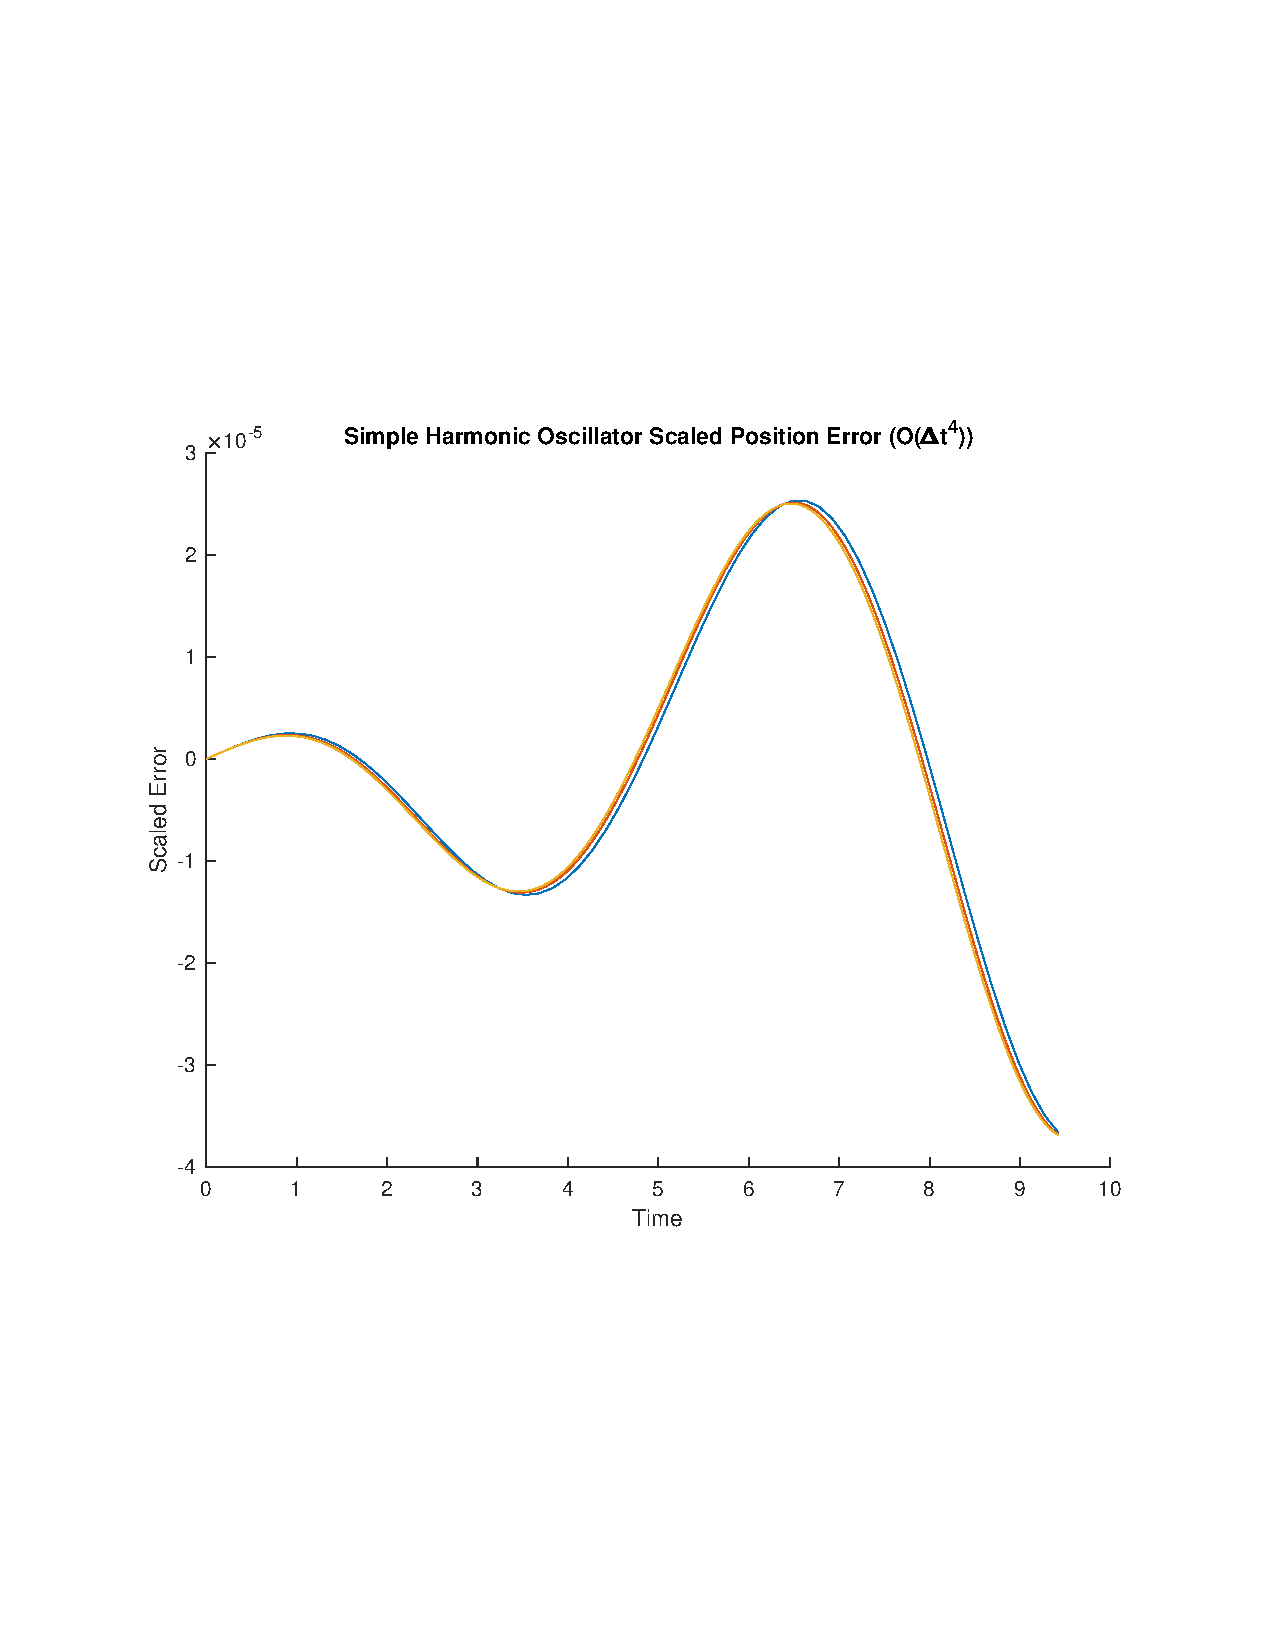
\includegraphics[width=10cm, height=8cm]{figures/sho_scaledErrors.pdf}
\end{figure}
\\
Below also included is the non-scaled errors which just proves the reason for needing to scale and justifies our determination that the scaling is required and thus that the solution is indeed $(O(\Delta t^4))$.\\
\begin{figure}[!h]
    \centering
    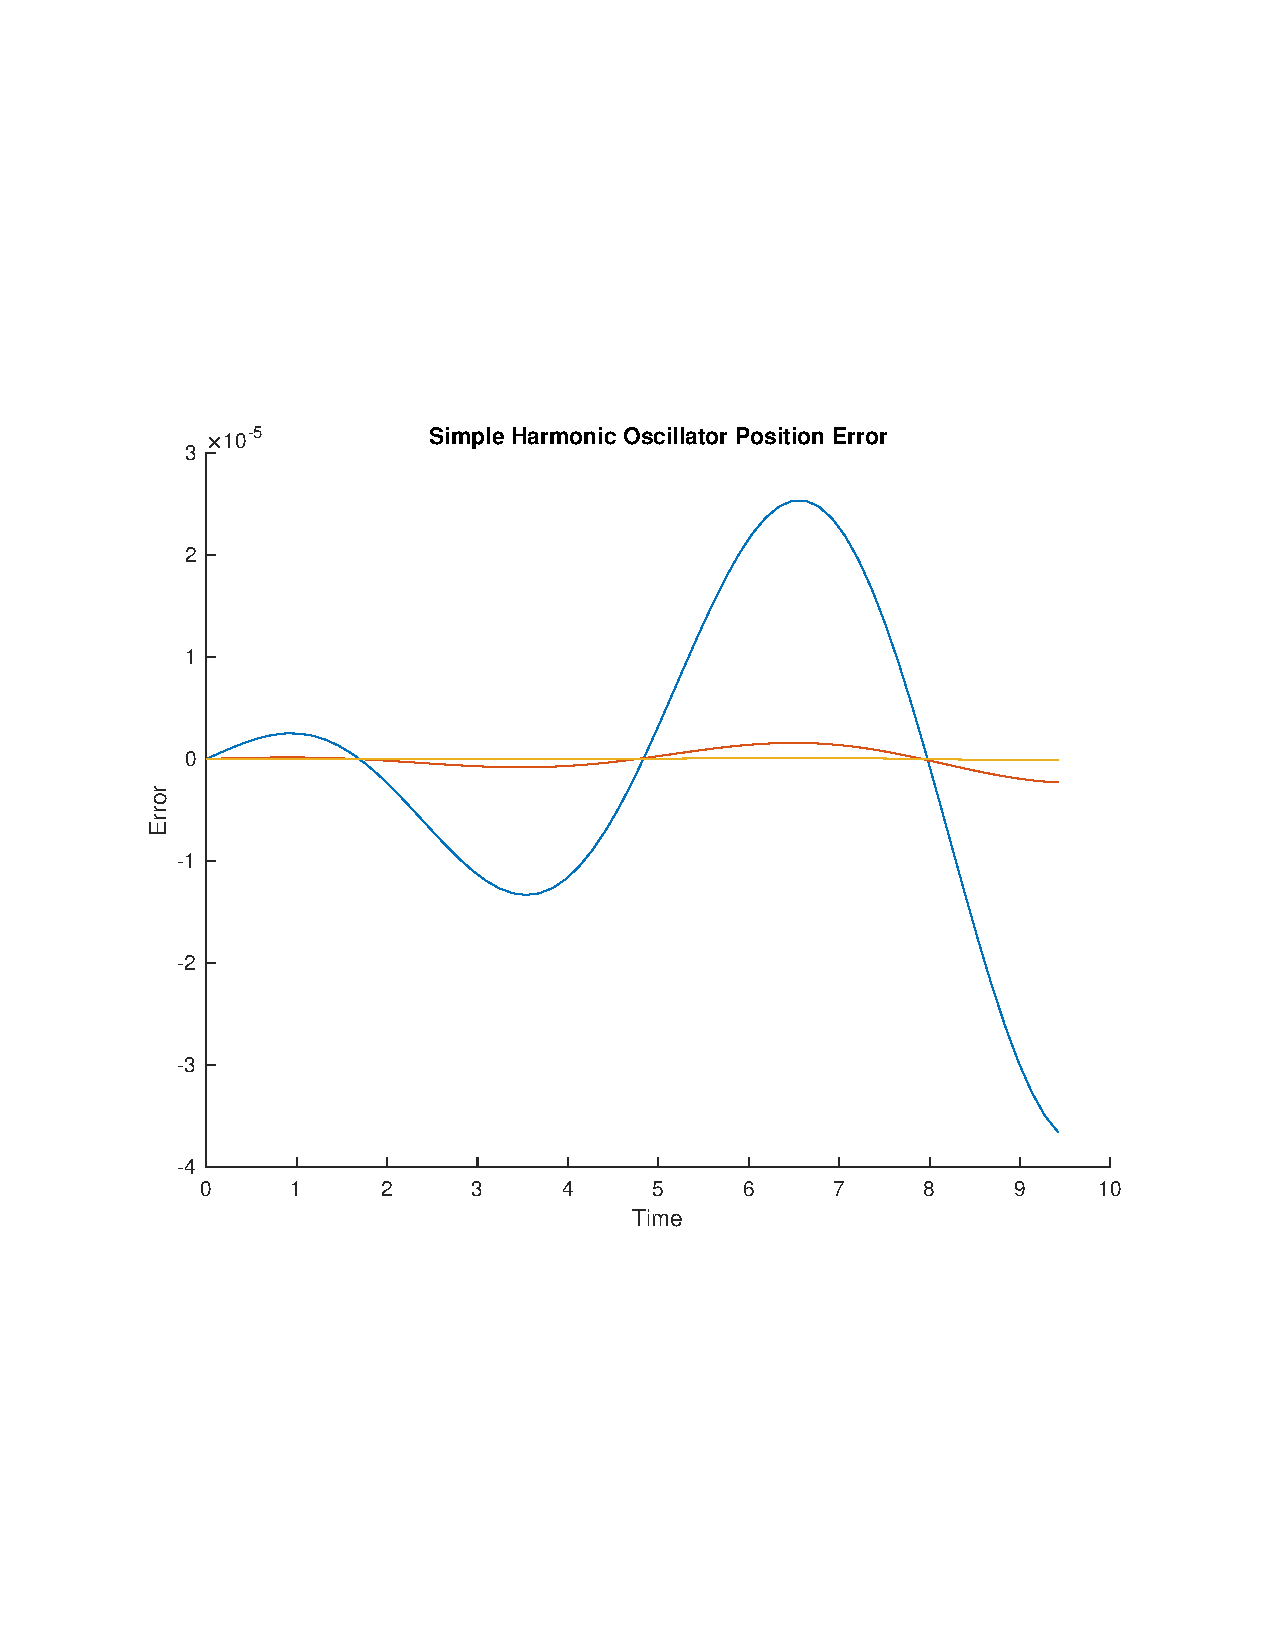
\includegraphics[width=10cm, height=7.5cm]{figures/sho_nonScaledErrors.pdf}
\end{figure}

\subsubsection{Van der Pol Oscillator}
The second part of this problem was analyzing the Van der Pol oscillator which was earlier briefly discussed in section 2.3. There were two objectives for this section which were plotting the position versus time as well as the phase space evolution. \\
\\
The ODE and the corresponding initial conditions for this problem were:
\begin{align*}
    & \frac{d^2x}{dt^2} + a(x^2-1) \frac{dx}{dt} + x = 0\\
    & x(0) = 1\\
    & \frac{dx}{dt}(0) = -6
\end{align*}
The application of our RK4 method for this resulted in the plots below:
\begin{figure}[!h]
    \centering
    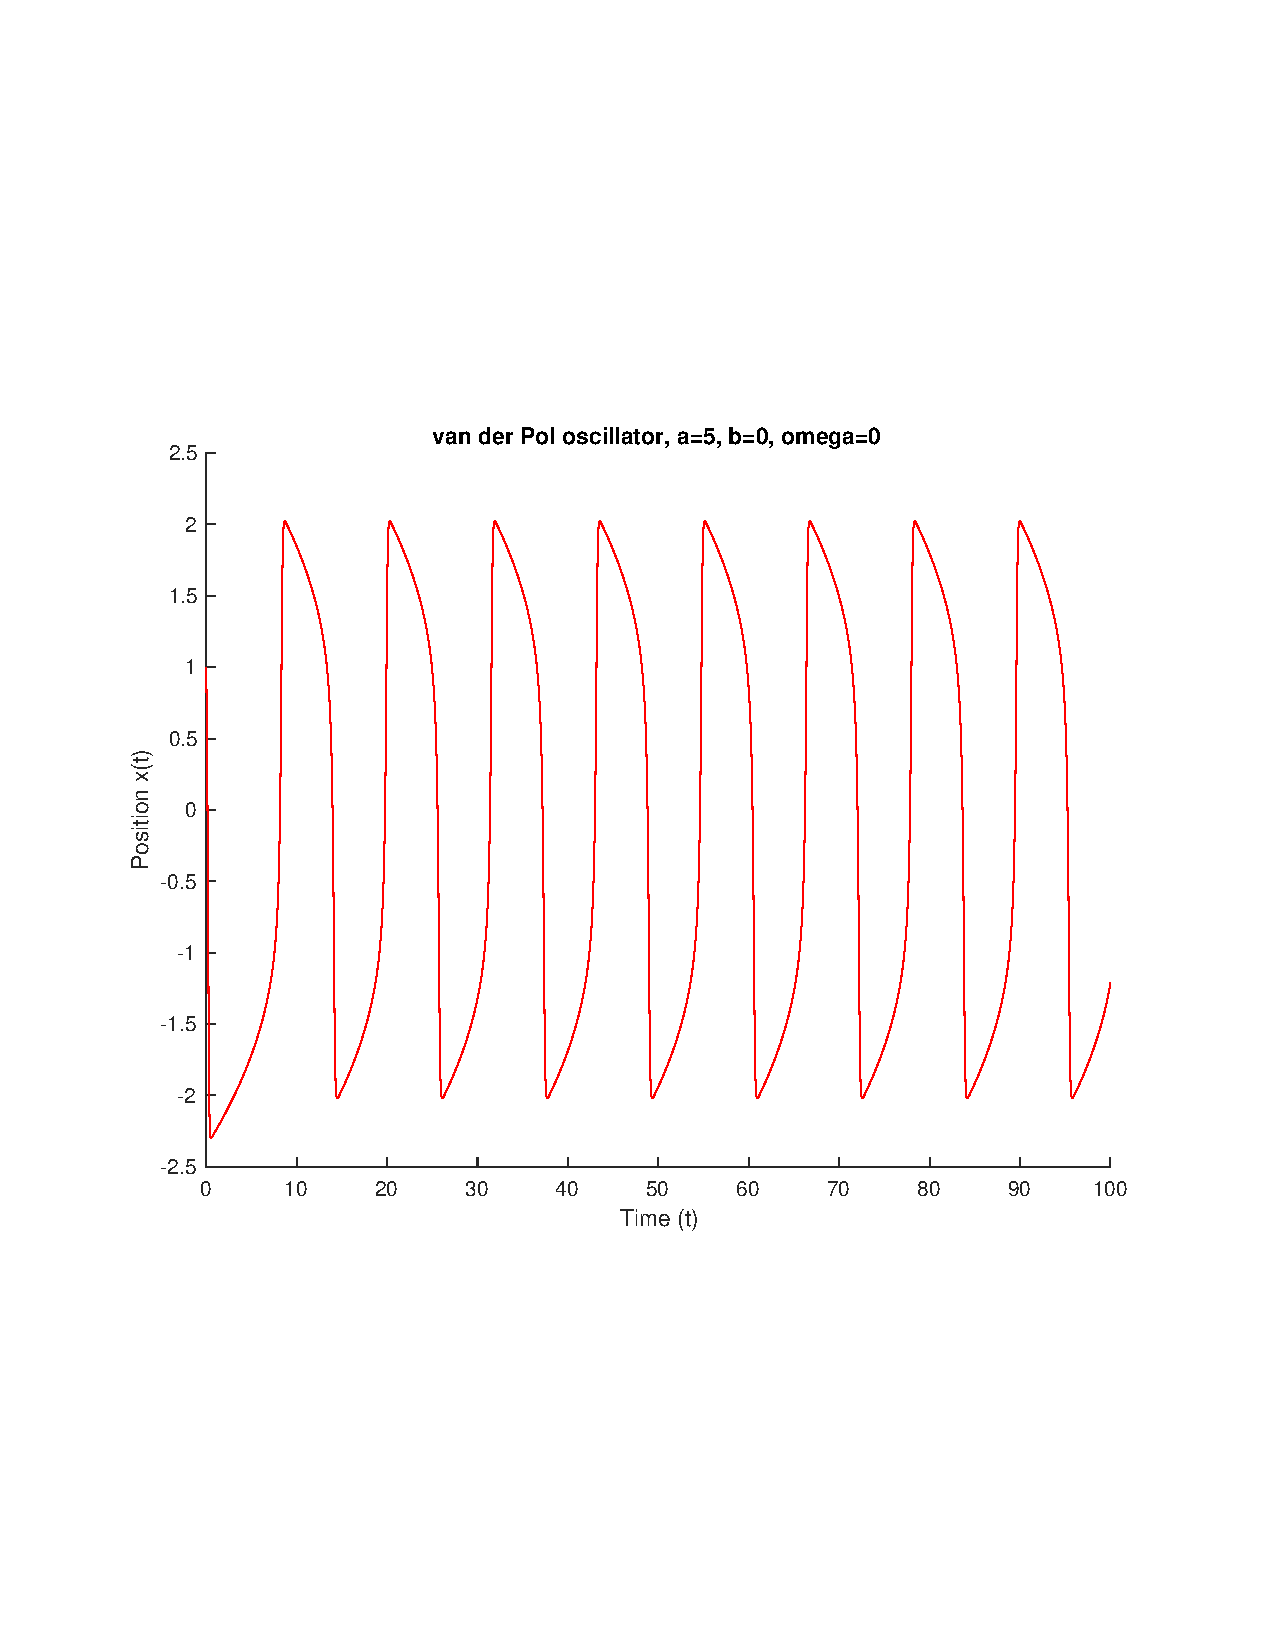
\includegraphics[width=10cm, height=7.5cm]{figures/vdp_Position.pdf}
\end{figure}
\begin{figure}[!h]
    \centering
    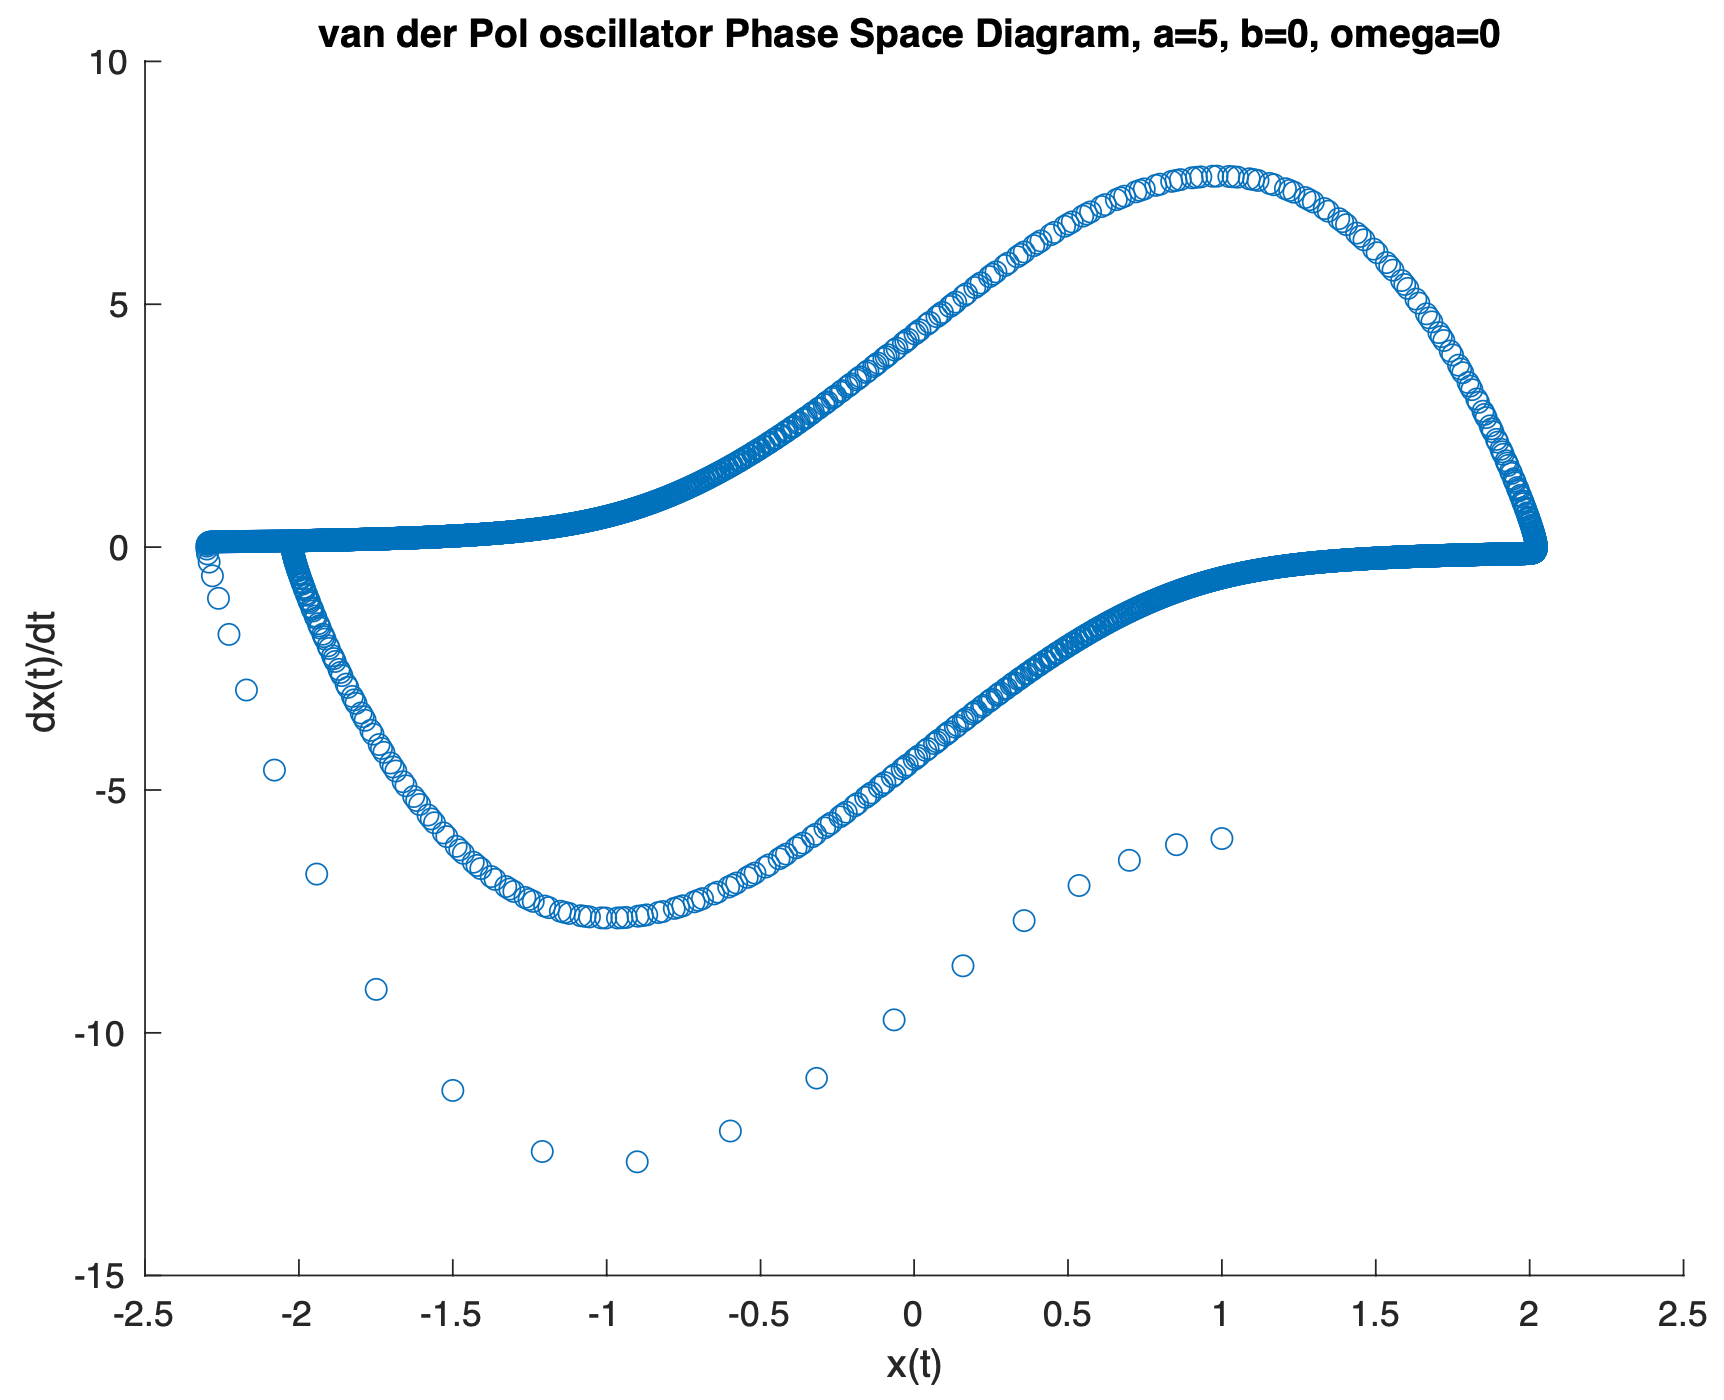
\includegraphics[width=10cm, height=7cm]{figures/vdp_phaseSpace.png}
\end{figure}
\\

\subsection{Problem 3}
For problem three the calculations and experiments were similar to that of problem two however using the new adaptive step size RK4 method.\\

\subsubsection{Simple Harmonic Oscillator (Adaptive RK4)}
The first experiment was calculating the errors compared to the analytical solution for different relative tolerances. Here we used reltol = [1.0e-5, 1.0e-7, 1.0e-9, 1.0e-11] for each different plot and took the results minus the analytical solution of the simple harmonic oscillator. We can see that the results mimic that of the non-scaled errors in problem two.\\
\\
One interesting observation for this plot is that the two plots which are closest to coincidence is when reltol is 1.0e-5 and 1.0e-11. This is could be to do with the initial rate at which a suitable $\Delta t$ was found. Since we also notice that the errors from the initial point for reltol is 1.0e-7 and 1.0e-9 quickly disperse to a higher amplitude waveform from the initial error of zero. One way to account for this might be a better guess for the first $\Delta t$ on those relative tolerances.
\begin{figure}[!h]
    \centering
    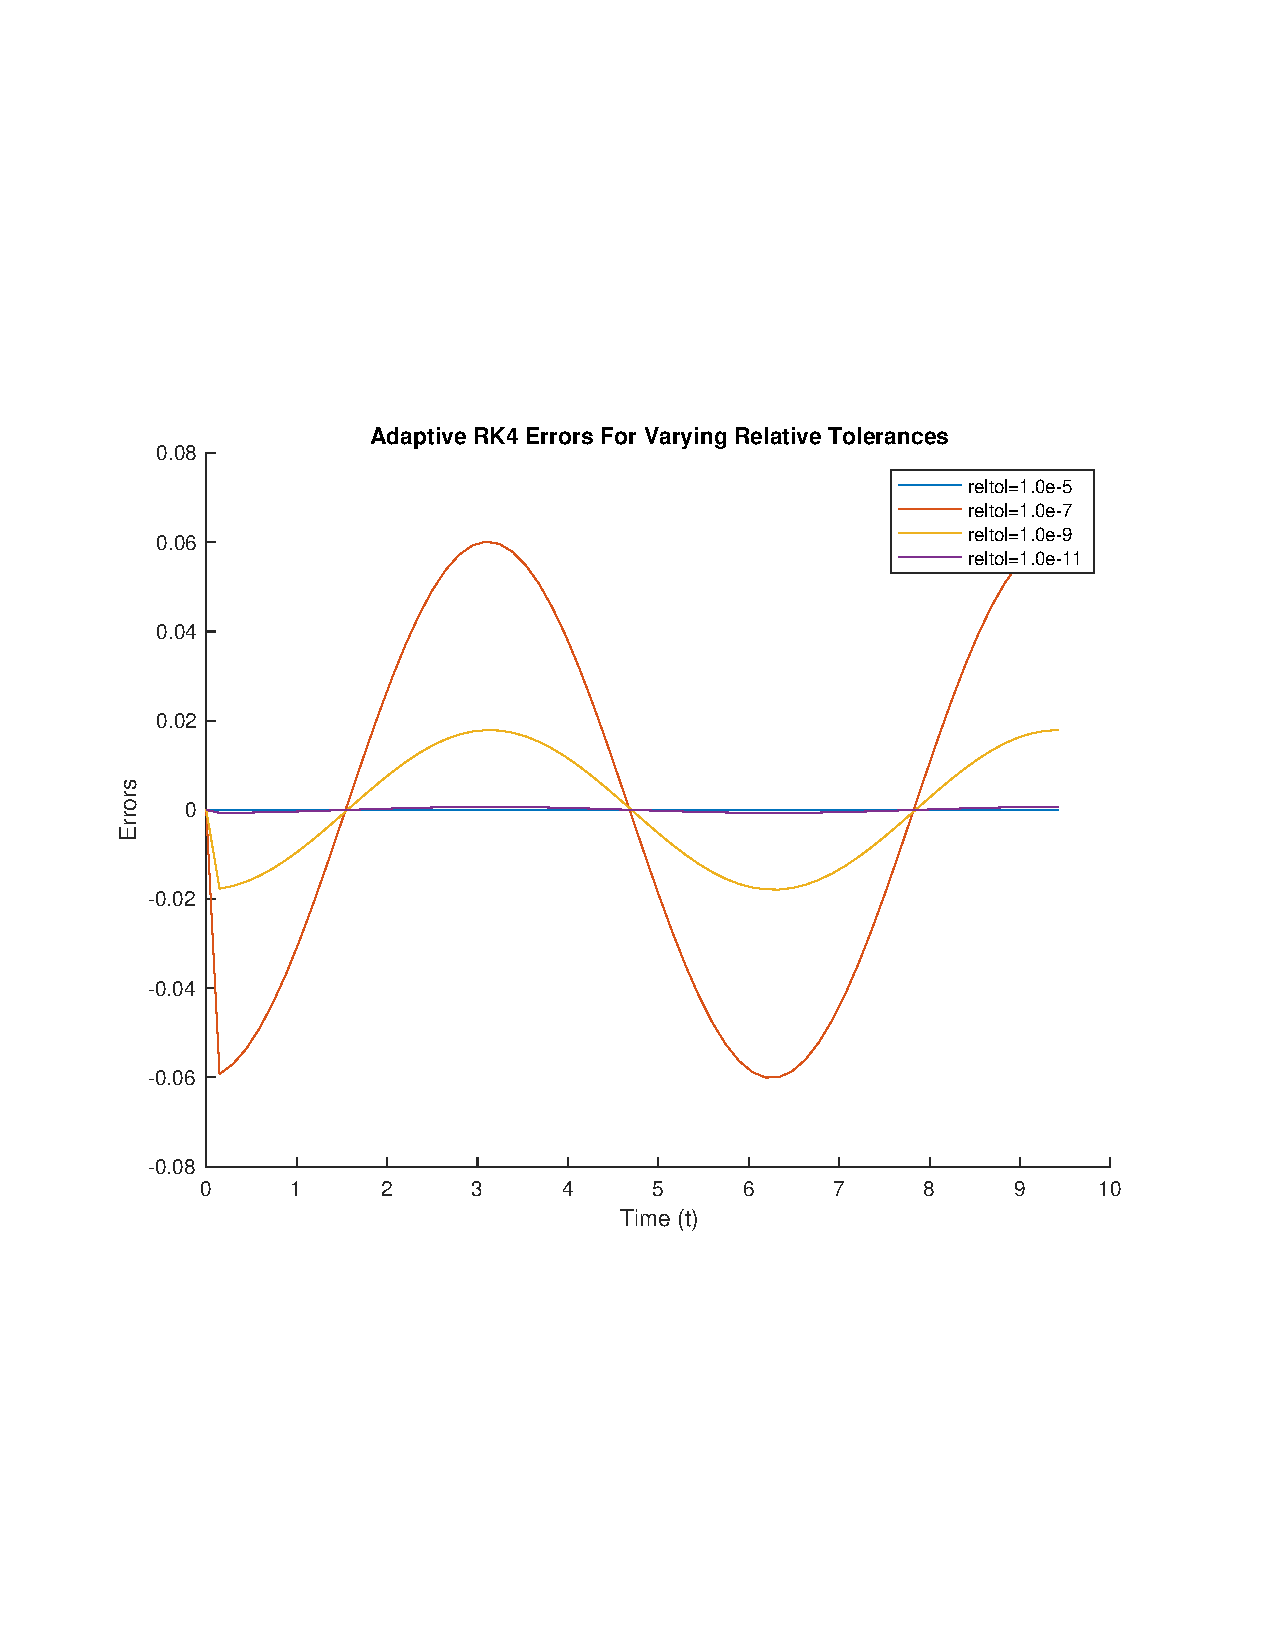
\includegraphics[width=10cm, height=7.2cm]
    {figures/adaptiveRK4_sho_err.pdf}
\end{figure}

\subsubsection{Van der Pol  Oscillator (Adaptive RK4)}
The final set of experiments in this homework were plotting the position versus time and phase space evolution for the Van der Pol oscillator using our adaptive RK4 integrator.\\
\\
The differences between these figures are quite minimal when compared to the normal RK4 integrator especially for the position versus time diagrams.\\
\\ 
However, one thing which can be identified in the phase space evolution is that the evenness of our points is not as smooth when compared to the basic RK4 integrator.for example especially at the top right portion of the graph you can see a greater dispersion between points at these sections.\\
\\
This would likely be a result of our adaptive step sizes which are easily visible here due to the variability in that space and displays our adaptive step sizes at work.
\begin{figure}[!h]
    \centering
    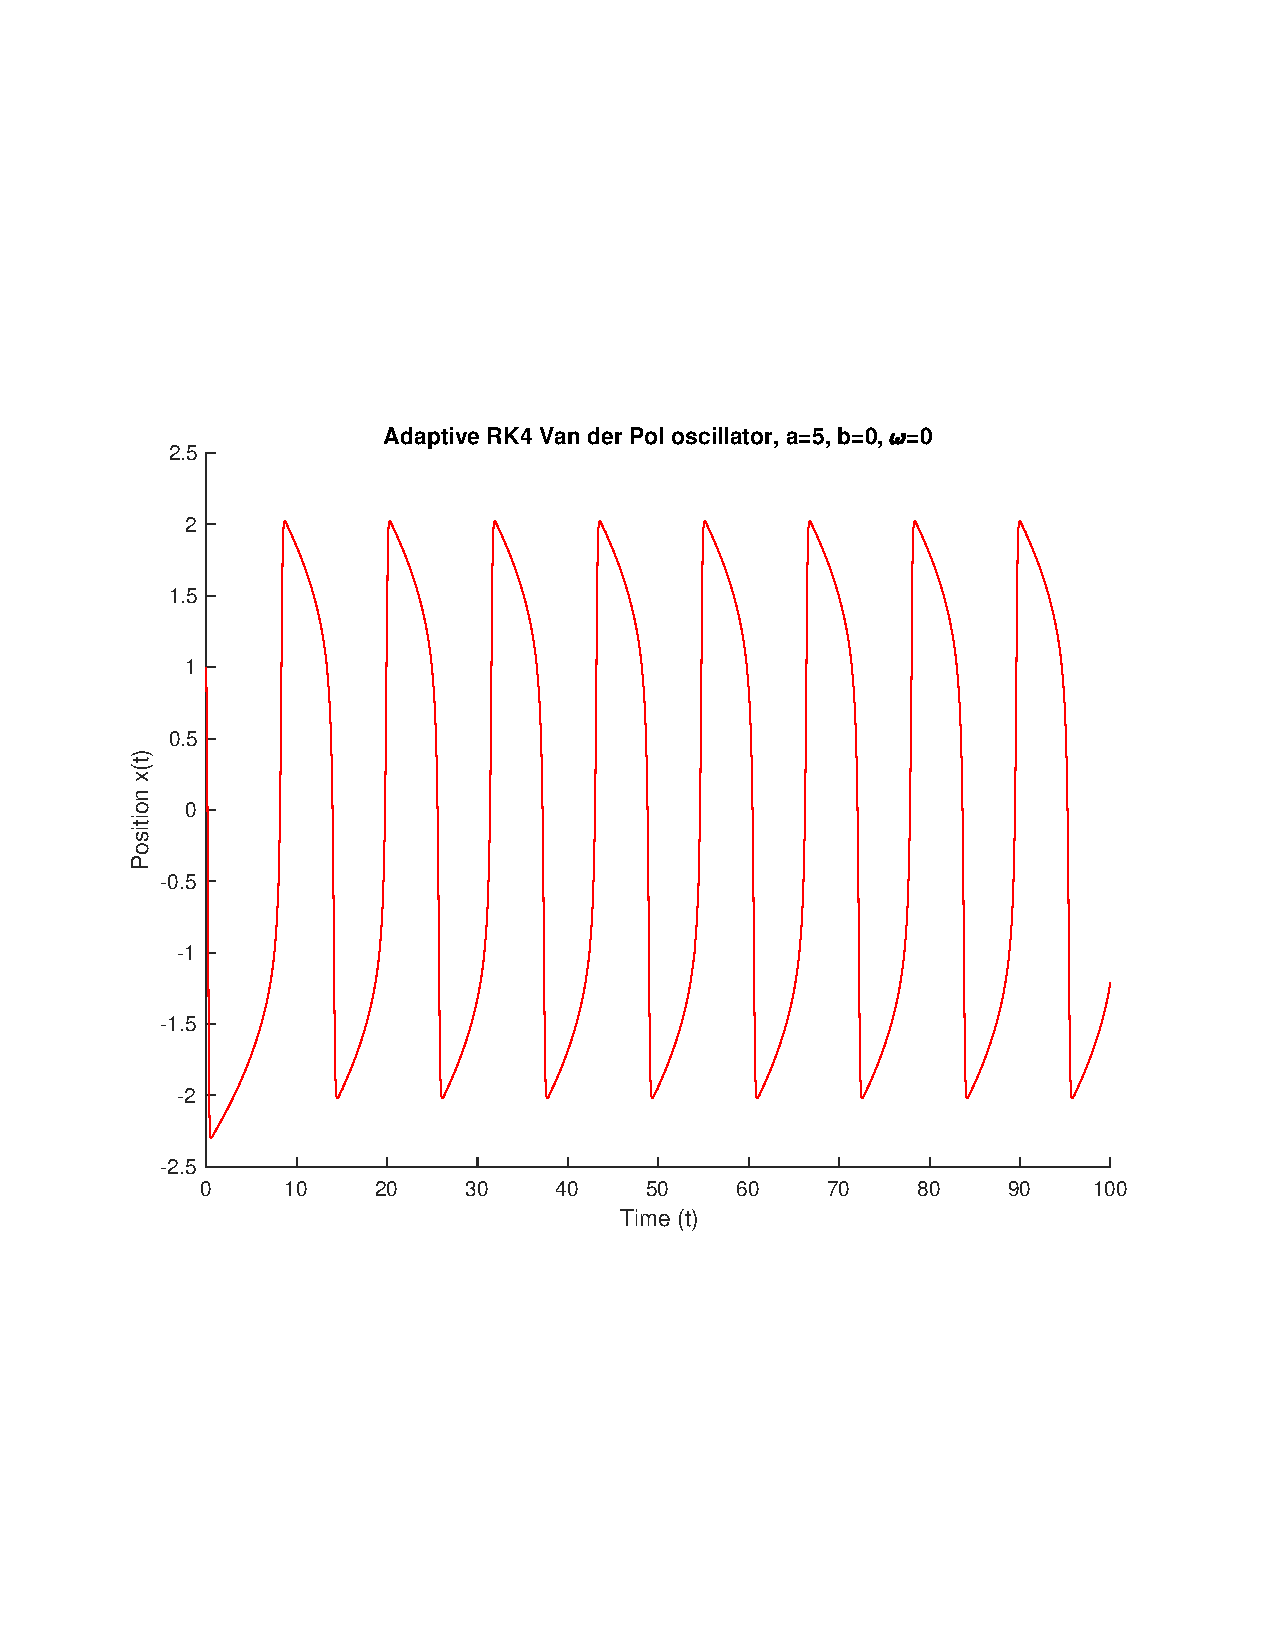
\includegraphics[width=10cm, height=8cm]
    {figures/adaptiveRK4_vdp_pos.pdf}
\end{figure}
\begin{figure}[!h]
    \centering
    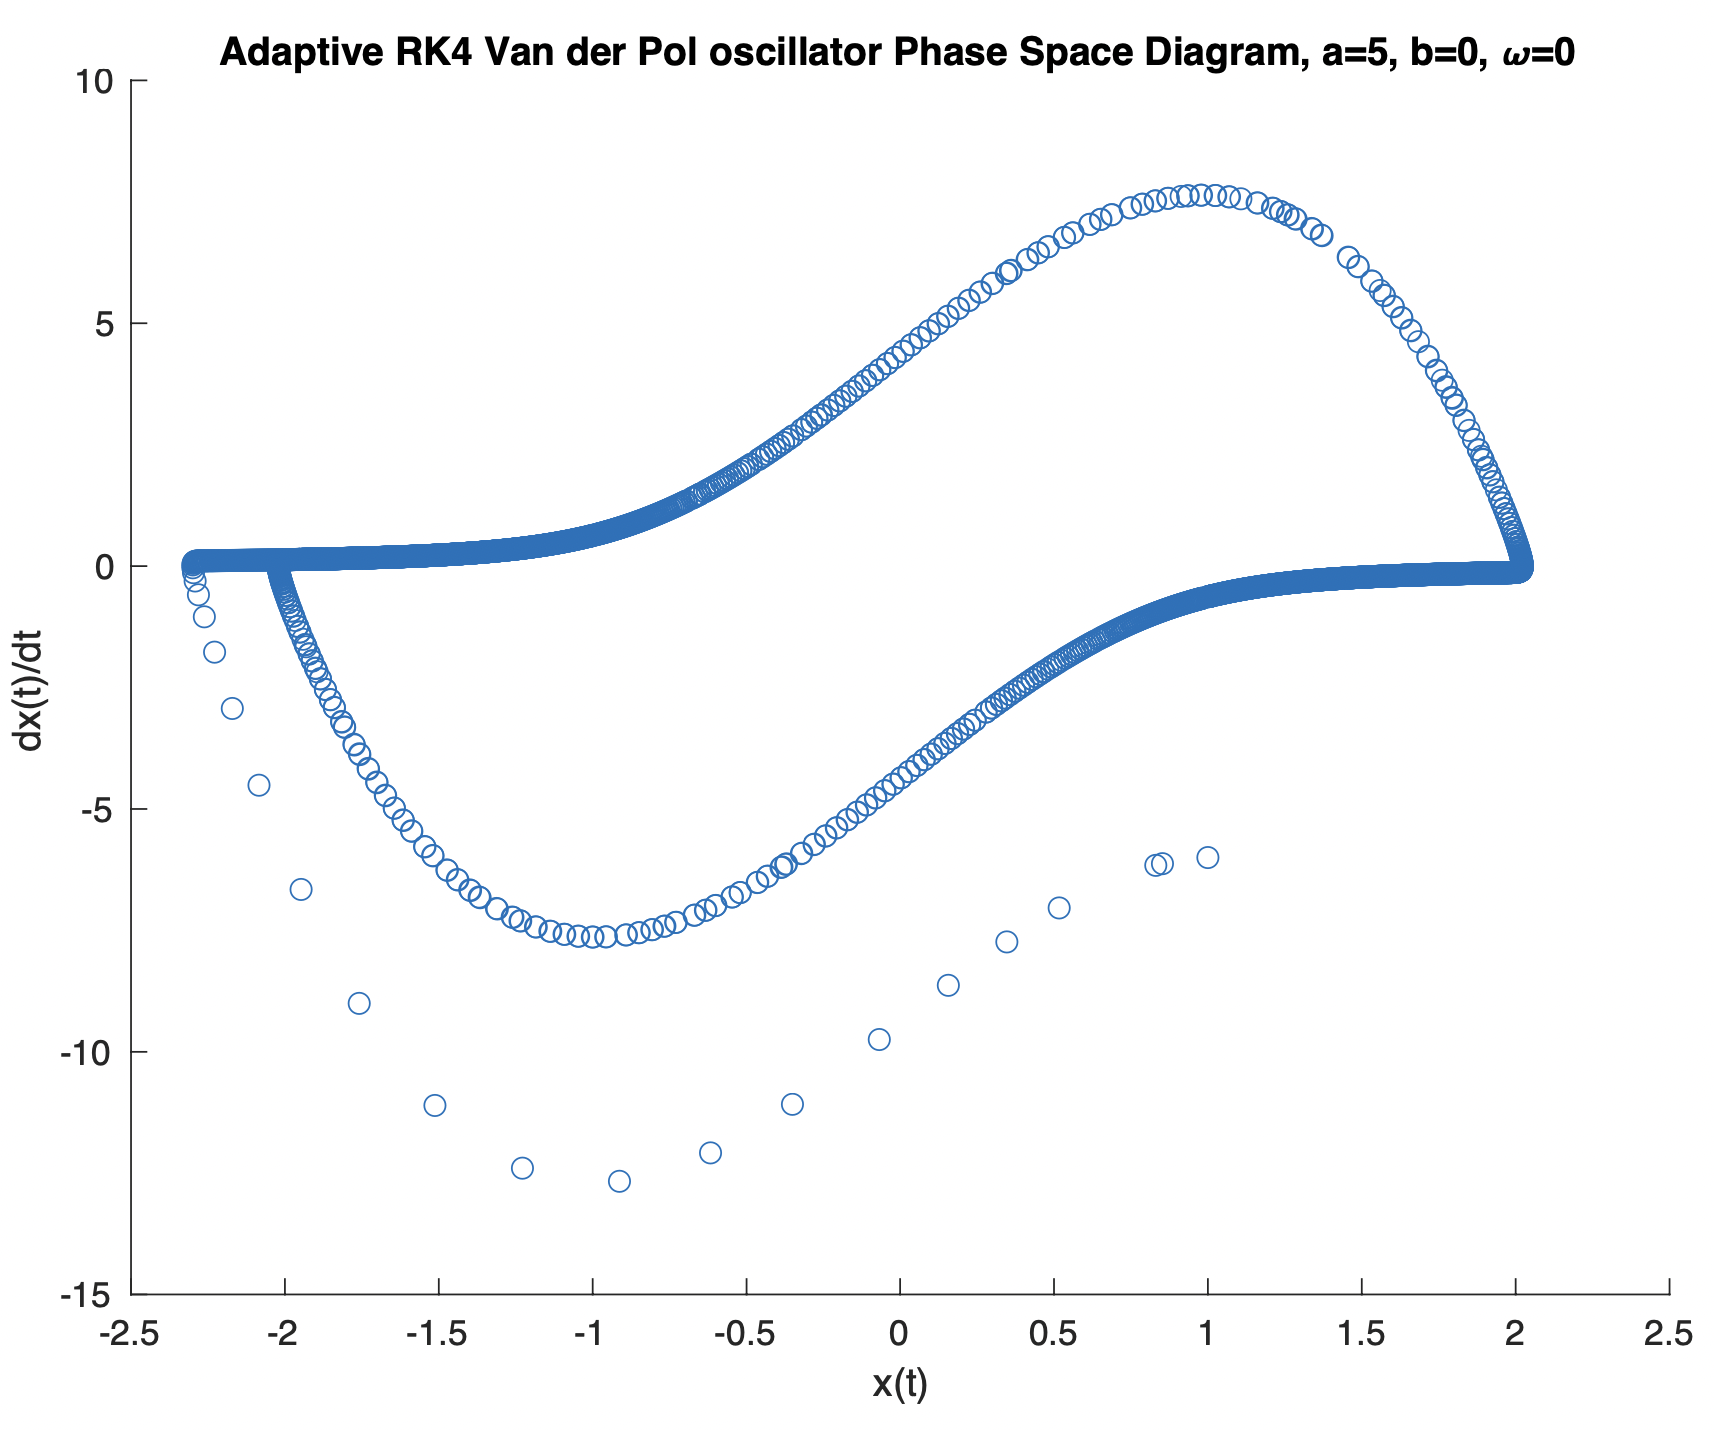
\includegraphics[width=10cm, height=7.5cm]
    {figures/adaptiveRK4_phaseSpace.png}
\end{figure}

\section{Conclusion}
Through this homework a variety of fourth order Runge-Kutta methods were investigated. Beginning with a single step we found and proved that the per step error was of fifth order for the fourth order Runge-Kutta method through a step of the simple harmonic oscillator. Moving onto the second problem we implemented our step function to build a full RK4 integrator which could be applied to provide a full solution. Lastly, an adaptive step size integrator was developed which provided another solution to these types of integrators. To verify and validate these methods we applied them onto the simple harmonic oscillator and the Van der Pol Oscillator plotting errors for the SHO and both the position versus time and the phase space evolution for the VDP oscillator.
\end{document}